\documentclass[11pt]{article}

\usepackage[margin=1in]{geometry}
\usepackage{setspace}
\usepackage{microtype}
\usepackage[T1]{fontenc}
\usepackage{lmodern}

\usepackage{amsmath, amssymb}
\usepackage{booktabs}
\usepackage{array}
\usepackage{multirow}
\usepackage{graphicx}
\usepackage{caption}
\usepackage{subcaption}
\usepackage{float}
\usepackage{siunitx}
  \sisetup{group-separator={,}, group-minimum-digits=4}

\usepackage[round, authoryear]{natbib}
\usepackage[hidelinks]{hyperref}

\title{\vspace{-1.5cm}\textbf{The Effects of 401(k) Participation on Household Wealth:\\
A Machine-Learning Approach}}
\author{%
  [Author 1] \and [Author 2] \and [Author 3] \and [Author 4] \\[2pt]
  \small \texttt{[email1@gatech.edu]} \quad
         \texttt{[email2@gatech.edu]} \quad
         \texttt{[email3@gatech.edu]} \quad
         \texttt{[email4@gatech.edu]}\\[6pt]
  \small Economics 4161/8803 -- Machine Learning for Economics \\
  \small Georgia Institute of Technology
}
\date{May 6, 2026}

\onehalfspacing

\begin{document}

\begin{titlepage}
  \maketitle
  \thispagestyle{empty}
  \vspace{0.5cm}

  \begin{center}
    \textbf{Abstract}
  \end{center}

  \noindent
  We study the causal effect of 401(k) participation on household wealth using
  the 1991 Survey of Income and Program Participation (SIPP).  Because
  participation is non-randomly chosen, we use 401(k) eligibility as an
  instrument and combine it with a flexible machine-learning estimator --- the
  instrumental forest of \cite{athey2019grf} --- trained on an 80/20
  train/test split.  The estimated average treatment effect on net financial
  assets is roughly \$11{,}400 (s.e.\ \$1{,}600), and on total wealth roughly
  \$9{,}700 (s.e.\ \$2{,}600).  Effects are positive across every income and
  education subgroup but rise sharply with income, and the divergence between
  net financial assets and total wealth in the upper income brackets is
  consistent with asset substitution.  These results are close to the OLS and
  2SLS estimates we obtain when replicating Panel A of Table~3 in
  \cite{ch2004}, supporting the substantive interpretation while showing how
  ML-based methods recover similar conclusions without imposing linearity.

  \vfill

  \noindent
  \textit{Acknowledgments.}  We thank [Instructor] and our classmates for
  helpful comments.  Code and data files for replication are submitted with
  this report.  Any remaining errors are our own.
\end{titlepage}

\setcounter{page}{1}

\section{Introduction}

The U.S.\ tax code subsidises private retirement saving through several
vehicles, of which 401(k) plans are among the most widely used.  Whether
these plans \emph{actually} raise household wealth, however, is a long-running
empirical question: workers with stronger preferences for saving may both
self-select into participation and accumulate more assets through other
channels, so any cross-sectional comparison of participants and
non-participants conflates the causal effect with selection bias
\citep{ch2004}.  A standard solution is to use 401(k) \emph{eligibility} ---
which depends on the employer's plan offering rather than the worker's
choice --- as an instrument for participation.

This project asks how much of the wealth gap between participants and
non-participants in the 1991 SIPP is causal, using a machine-learning
estimator of the treatment effect and comparing it to traditional OLS and
2SLS regressions.  We focus on three measures of wealth used in
\cite{ch2004}: net financial assets (NFA), net non-401(k) financial assets
(NNFA), and total wealth (TW).  Throughout, we use 401(k) eligibility
(\texttt{e401}) as an instrument for participation (\texttt{p401}).

Our empirical approach has three parts.  First, we estimate a random forest
that predicts wealth from a vector of demographic and household variables;
this gives us a flexible benchmark for predictive accuracy and a sense of
which variables matter.  Second, we estimate average and individual-level
treatment effects using the instrumental forest of \cite{athey2019grf}, a
non-parametric IV estimator that allows the treatment effect to vary with
covariates.  Third, we replicate the OLS and 2SLS estimates in Panel~A of
Table~3 of \cite{ch2004} on the full sample and within seven income brackets,
and compare them to our ML estimates.

The main results are as follows.  The instrumental forest yields an average
treatment effect of about \$11{,}400 on net financial assets and \$9{,}700 on
total wealth.  These estimates are statistically significant, similar in
magnitude to the 2SLS estimates from the replication (\$13{,}087 and \$9{,}259
respectively), and clearly below the corresponding OLS estimates --- consistent
with the upward selection bias emphasised in the prior literature.  The
treatment effect rises monotonically with income, more than doubling between
the bottom and top brackets, and is also higher for more educated households.
The estimated effect on net financial assets exceeds the effect on total
wealth at high incomes, suggesting that some of the additional 401(k) wealth
is offset by reductions in other forms of wealth at the top of the
distribution --- the same substitution pattern documented by \cite{ch2004}
using instrumental quantile regression.

The rest of the paper proceeds as follows.  Section~\ref{sec:data} describes
the data.  Section~\ref{sec:methods} explains the methodology.
Section~\ref{sec:results} reports the ML and replication results and
compares them.  Section~\ref{sec:conclusion} concludes with a discussion of
caveats.

\section{Data}\label{sec:data}

\paragraph{Sample.}
The data come from the 1991 wave of the Survey of Income and Program
Participation (SIPP), restricted as in \cite{ch2004} to households with at
least one employed but no self-employed person, with a household reference
person aged 25--64.  The resulting sample contains
$N = 9{,}915$ households.  We use the dataset \texttt{401k.csv} provided
with the assignment.  Variable definitions are taken from the accompanying
codebook.  We do no imputation: the data have no missing values on the
variables we use.  Summary statistics are reported in Table~\ref{tab:summary}.

\paragraph{Variables.}
The outcome of primary interest is net financial assets (\texttt{net\_tfa}).
To check robustness and study substitution, we also study net non-401(k)
financial assets (\texttt{net\_nifa}) and total wealth (\texttt{tw}).  The
treatment is 401(k) participation (\texttt{p401}); the instrument is 401(k)
eligibility (\texttt{e401}).  Covariates used in all specifications are: age
and four age-bracket dummies ($<\!30$, 30--35, 36--44, 45--54, with 55+ as
base); income (\texttt{inc}) and six income-bracket dummies (with $<\!\$10$K
as base); family size; an indicator for being married; an indicator for
two-earner households; an indicator for having a defined-benefit pension; an
indicator for IRA participation; an indicator for home ownership; and three
education dummies (high school, some college, college+, with no high school
as base).  Income enters as a continuous variable in the within-bracket
regressions described in Section~\ref{sec:methods}.

\paragraph{Descriptive patterns.}
Several features of the data motivate the analysis.  First, participants
hold substantially more wealth than non-participants on every measure: mean
net financial assets are about \$38{,}000 for participants versus \$11{,}000
for non-participants, and mean total wealth is roughly \$97{,}000 versus
\$52{,}000.  Second, participants differ systematically from non-participants
on observable characteristics that are themselves correlated with wealth:
they have higher income (\$49{,}000 vs.\ \$33{,}000), are more likely to be
married (69\% vs.\ 57\%), more likely to own a home (77\% vs.\ 59\%), and
more likely to hold an IRA (36\% vs.\ 20\%).  These differences make a naive
participant-vs-nonparticipant comparison unreliable as a causal estimate.

\paragraph{Eligibility as an instrument.}
The unconditional participation rate is 26.2\% and the eligibility rate is
37.1\%; among eligible workers, 70.6\% participate.  In the regressions
reported below, the first-stage coefficient on \texttt{e401} when
\texttt{p401} is regressed on the full set of controls is 0.697 (\textit{F}
greatly above the conventional weak-instrument threshold), confirming that
eligibility strongly predicts participation conditional on covariates.

\begin{table}[H]
  \centering
  \caption{Summary statistics, 1991 SIPP analysis sample.}
  \label{tab:summary}
  \footnotesize
  \begin{tabular}{l S[table-format=6.0] S[table-format=6.0] S[table-format=6.0] S[table-format=6.0]}
    \toprule
    & \multicolumn{2}{c}{Full sample} & {Participants} & {Non-Participants} \\
    \cmidrule(lr){2-3}\cmidrule(lr){4-4}\cmidrule(lr){5-5}
    Variable & {Mean} & {Std.\ Dev.} & {Mean} & {Mean} \\
    \midrule
    Net financial assets (\$)            &  18052 &  63522 & 38262 & 10890 \\
    Net non-401(k) financial assets (\$) &  10414 &  56029 & 17270 &  7985 \\
    Total wealth (\$)                    &  63817 & 111530 & 96920 & 52088 \\
    Income (\$)                          &  37201 &  24774 & 49367 & 32890 \\
    Age                                  &     41 &     10 &    42 &    41 \\
    Family size                          &      3 &      2 &     3 &     3 \\
    Married                              &   0.60 &   0.49 &  0.69 &  0.57 \\
    IRA participant                      &   0.24 &   0.43 &  0.36 &  0.20 \\
    Defined-benefit pension              &   0.27 &   0.44 &  0.39 &  0.23 \\
    Home owner                           &   0.64 &   0.48 &  0.77 &  0.59 \\
    Education: no high school            &   0.13 &   0.33 &  0.07 &  0.15 \\
    Education: high school               &   0.38 &   0.48 &  0.35 &  0.39 \\
    Education: some college              &   0.24 &   0.43 &  0.26 &  0.24 \\
    Education: college+                  &   0.25 &   0.43 &  0.33 &  0.22 \\
    \midrule
    Observations & {9{,}915} & & {2{,}594} & {7{,}321} \\
    \bottomrule
  \end{tabular}
  \par\smallskip
  \footnotesize
  \textit{Notes.}  Source: 1991 Survey of Income and Program Participation.
  Sample is restricted to households with at least one employed but no
  self-employed worker, head aged 25--64.  Participation = 401(k)
  participation; eligibility statistics not shown.  Wealth variables in
  current 1991 dollars.
\end{table}

Figure~\ref{fig:wealthdist} contrasts the distributions of the three wealth
measures by participation status, winsorised at the 5th and 95th percentiles
for visual clarity.  Participants' distributions are visibly shifted to the
right.  Figure~\ref{fig:wealthinc} shows that this gap widens with income.

\begin{figure}[H]
  \centering
  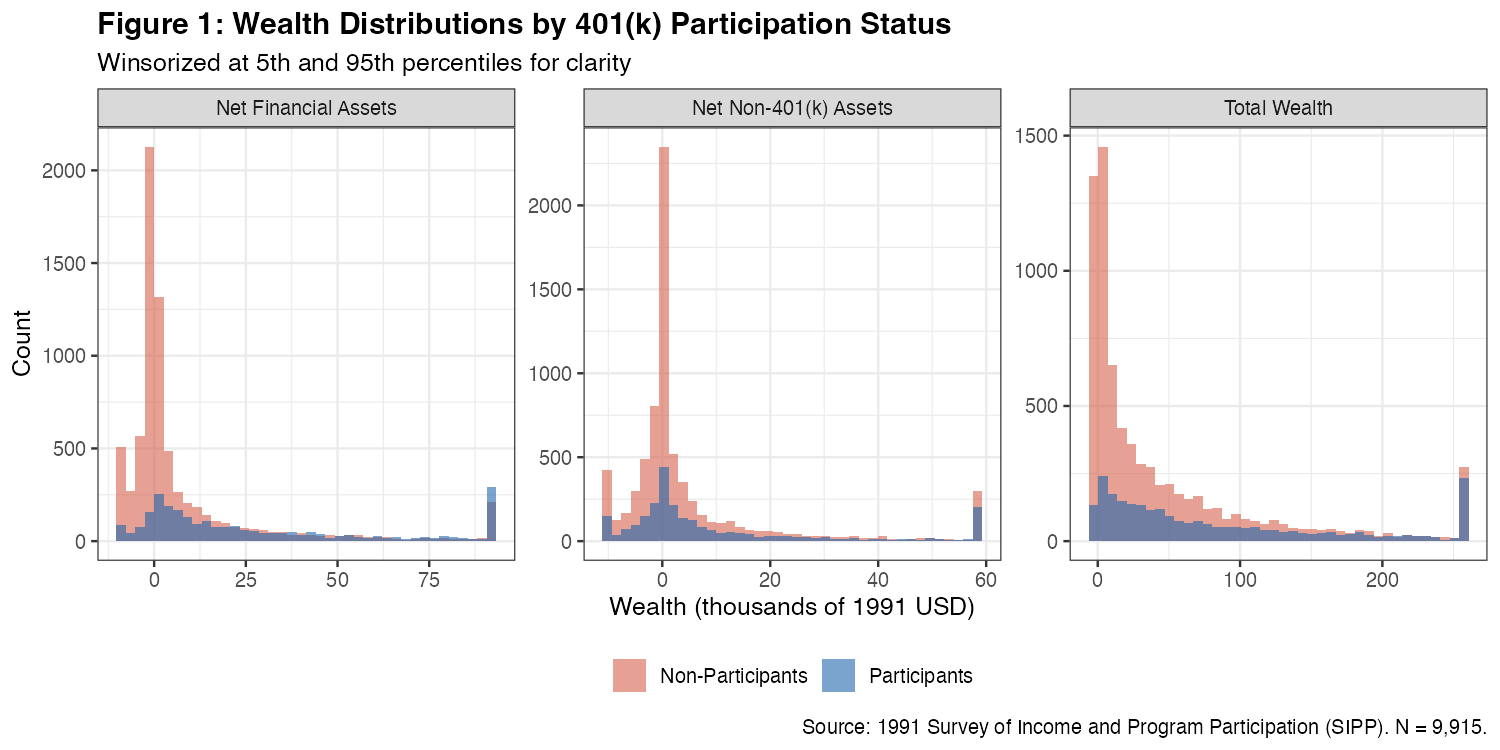
\includegraphics[width=0.85\linewidth]{figure1_wealth_distributions.png}
  \caption{Wealth distributions by 401(k) participation status (winsorised at
  the 5th and 95th percentiles for legibility).  Source: 1991 SIPP,
  $N=9{,}915$.}
  \label{fig:wealthdist}
\end{figure}

\begin{figure}[H]
  \centering
  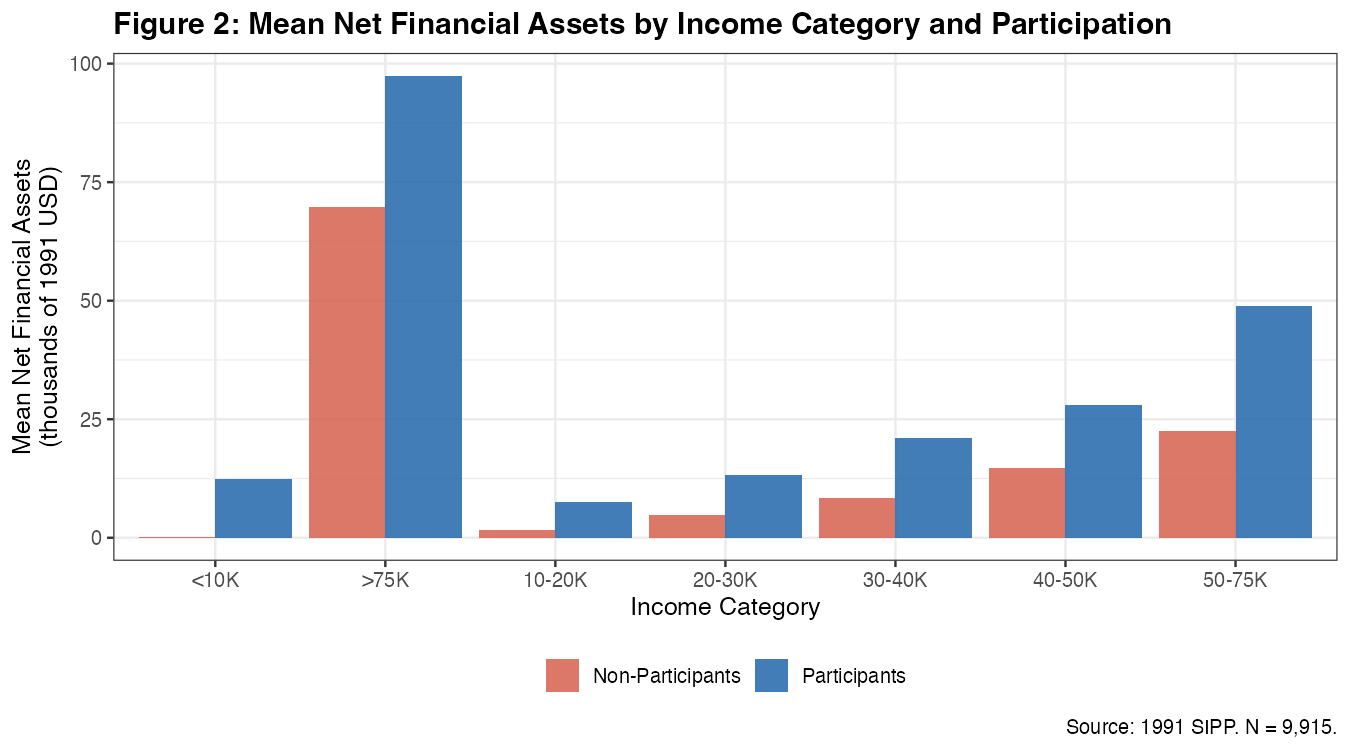
\includegraphics[width=0.85\linewidth]{figure2_wealth_by_income.png}
  \caption{Mean net financial assets by income bracket and 401(k)
  participation status.  Source: 1991 SIPP, $N=9{,}915$.}
  \label{fig:wealthinc}
\end{figure}

\section{Methods}\label{sec:methods}

\subsection{Why an instrumental ML estimator?}

A naive regression of wealth on participation overstates the causal effect
because of unobserved heterogeneity in the propensity to save: people who are
more inclined to save accumulate more wealth \emph{and} are more likely to
participate in any voluntary plan they have access to \citep{ch2004}.  The
standard fix is to use 401(k) eligibility, which is determined by the
employer's plan offering, as an instrument for participation.  Conditional on
income and other covariates, eligibility plausibly affects wealth only
through participation, satisfying the exclusion restriction.  This is the
identification strategy used in the linear 2SLS regressions we replicate
below.

We complement the parametric 2SLS with an instrumental forest
\citep{athey2019grf}, which estimates conditional local average treatment
effects $\tau(x) = \mathbb{E}[Y(1) - Y(0) \mid X = x, \text{complier}]$
non-parametrically.  Our motivation for choosing this method, rather than
e.g.\ a deeper neural net or boosted trees, is that:
(i) it directly produces individual-level treatment-effect estimates and a
valid average treatment effect, which is what we ultimately want;
(ii) it natively handles a binary instrument and binary treatment, removing
the need to bolt on a separate first stage;
(iii) it is robust to the kinds of nonlinearities and interactions among
demographics that one expects in wealth data; and
(iv) it does not require us to impose a parametric form for $\tau(x)$, so we
can study heterogeneity in the treatment effect by income, education, and age
without committing to interaction terms in advance.  For pure prediction
checks we use a standard random forest with default tuning.

\subsection{Modelling pipeline}

\paragraph{Train/test split.}
We split the 9{,}915 observations into a training set of 7{,}932
observations (80\%) and a test set of 1{,}983 observations (20\%) using a
fixed seed.  Hyperparameters are chosen using the training set only; all
performance and treatment-effect statistics reported below are evaluated on
the test set, so as to give a clean out-of-sample measure of model
performance and avoid in-sample overfitting bias in the estimated effects.

\paragraph{Random forest for prediction.}
We train two random forests --- one for net financial assets and one for total
wealth --- using the variables listed above plus \texttt{p401} as features
(\texttt{p401} is included here only because the goal is prediction, not
causal estimation).  We tune \texttt{mtry} by minimising the out-of-bag
mean-squared error on the training set, choosing among
$\{\sqrt{p}, p/4, p/3, p/2\}$.  The selected forests use 500 trees.  The
random forest provides a benchmark for predictive accuracy and a
permutation-based variable-importance ranking.

\paragraph{Instrumental forest for treatment effects.}
For causal estimation we use \texttt{instrumental\_forest()} from the
\texttt{grf} R package, with $Y$ equal to the outcome of interest, $W$ equal
to \texttt{p401}, and $Z$ equal to \texttt{e401}.  The covariate matrix $X$
contains all the controls listed in Section~\ref{sec:data} \emph{except}
\texttt{p401}.  We grow 2{,}000 trees and use the package's automatic tuning
of \texttt{min.node.size}, \texttt{sample.fraction}, \texttt{mtry} and other
splitting parameters.  The function \texttt{average\_treatment\_effect()}
returns the doubly-robust ATE estimator described in
\cite{athey2019grf}; we report this as the headline ML estimate.
Individual-level estimates $\hat\tau_i$ are then aggregated by income,
education, and age groups to study heterogeneity.

\subsection{Replication: OLS and 2SLS}

We replicate Panel~A of Table~3 of \cite{ch2004}.  For each of the three
wealth outcomes we estimate two specifications:
\begin{align}
  \text{OLS:}\quad & Y_i = \alpha + \beta \, \text{p401}_i + X_i^\top \gamma + \varepsilon_i, \label{eq:ols}\\
  \text{2SLS:}\quad & Y_i = \alpha + \beta \, \widehat{\text{p401}}_i + X_i^\top \gamma + \varepsilon_i, \label{eq:2sls}
\end{align}
where the first stage is
$\text{p401}_i = \pi_0 + \pi_1 \, \text{e401}_i + X_i^\top \pi_2 + u_i$.
The control vector $X_i$ contains the four age-bracket dummies, the six
income-bracket dummies, the three education dummies, and the household
covariates listed in Section~\ref{sec:data}.  In the by-income-bracket
regressions we drop the income-bracket dummies and instead include income
linearly, again following \cite{ch2004}.  We report robust (HC1) standard
errors throughout.

\section{Results and Replication Exercise}\label{sec:results}

\subsection{Random-forest prediction performance}

The random forest's out-of-sample performance on the test set is summarised
in Table~\ref{tab:perf}.  The model explains 29.1\% of the variation in net
financial assets and 46.2\% of the variation in total wealth, with root
mean-squared errors of about \$56{,}100 and \$88{,}300 respectively.  These
fits are not high in absolute terms --- wealth is notoriously hard to
predict, especially in the tails --- but they are comparable to what is
typically obtained on this dataset and are sufficient for the model to
function as a base learner inside the instrumental forest.

\begin{table}[H]
  \centering
  \caption{Random-forest predictive performance on test set ($n=1{,}983$).}
  \label{tab:perf}
  \begin{tabular}{l S[table-format=6.0] S[table-format=1.3]}
    \toprule
    Outcome & {RMSE (\$)} & {$R^2$} \\
    \midrule
    Net financial assets & 56102 & 0.291 \\
    Total wealth         & 88344 & 0.462 \\
    \bottomrule
  \end{tabular}
  \par\smallskip
  \footnotesize
  \textit{Notes.}  Random forest with 500 trees, \texttt{mtry} chosen by OOB
  error.  Train/test split: 7{,}932/1{,}983.  Outcome variables in 1991
  dollars.
\end{table}

The variable-importance ranking from the random forest
(Figure~\ref{fig:varimp}) places income at the top, followed by age and home
ownership.  This is consistent with intuition --- richer, older, and
home-owning households accumulate more financial assets --- and with the
specifications used in the replication regressions.  Predicted versus
actual values for net financial assets are plotted in
Figure~\ref{fig:fit}; the figure makes it visible that the model captures
the central tendency well but compresses the right tail, which is the major
source of residual variance.

\begin{figure}[H]
  \centering
  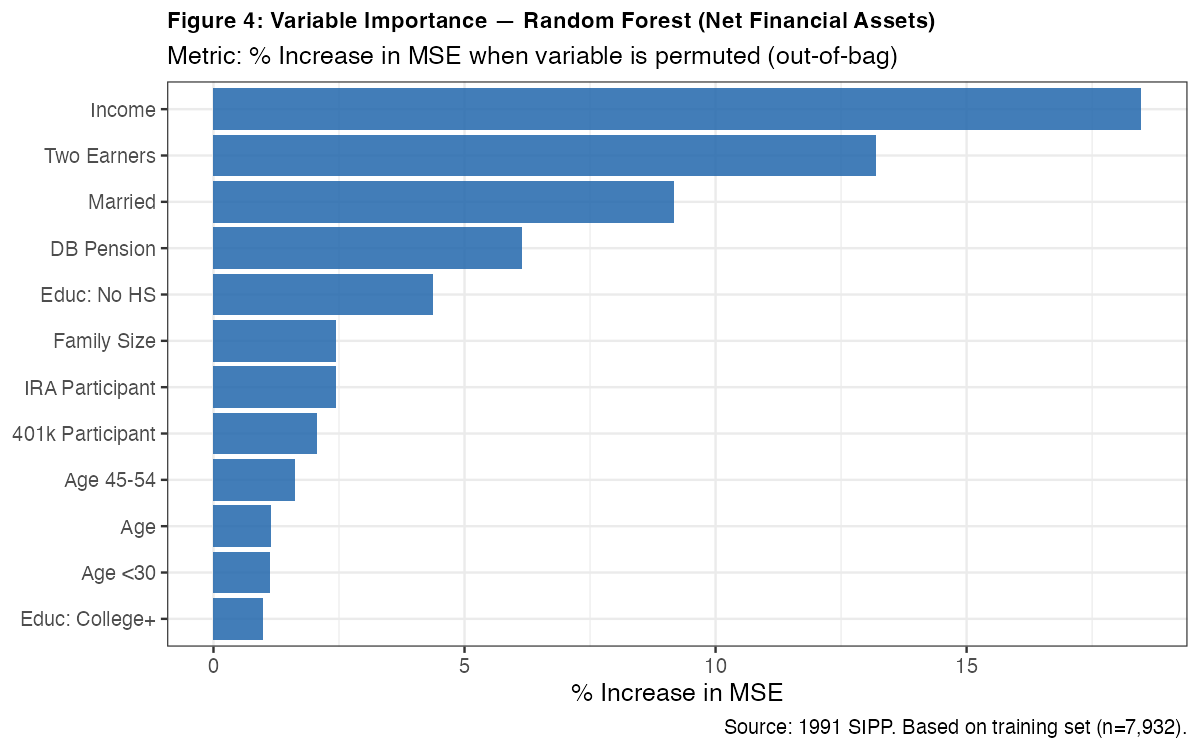
\includegraphics[width=0.75\linewidth]{figure4_variable_importance.png}
  \caption{Variable importance from the random forest predicting net
  financial assets, measured as the percentage increase in mean-squared
  error when the variable is permuted out of bag.  Source: 1991 SIPP
  training set ($n=7{,}932$).}
  \label{fig:varimp}
\end{figure}

\begin{figure}[H]
  \centering
  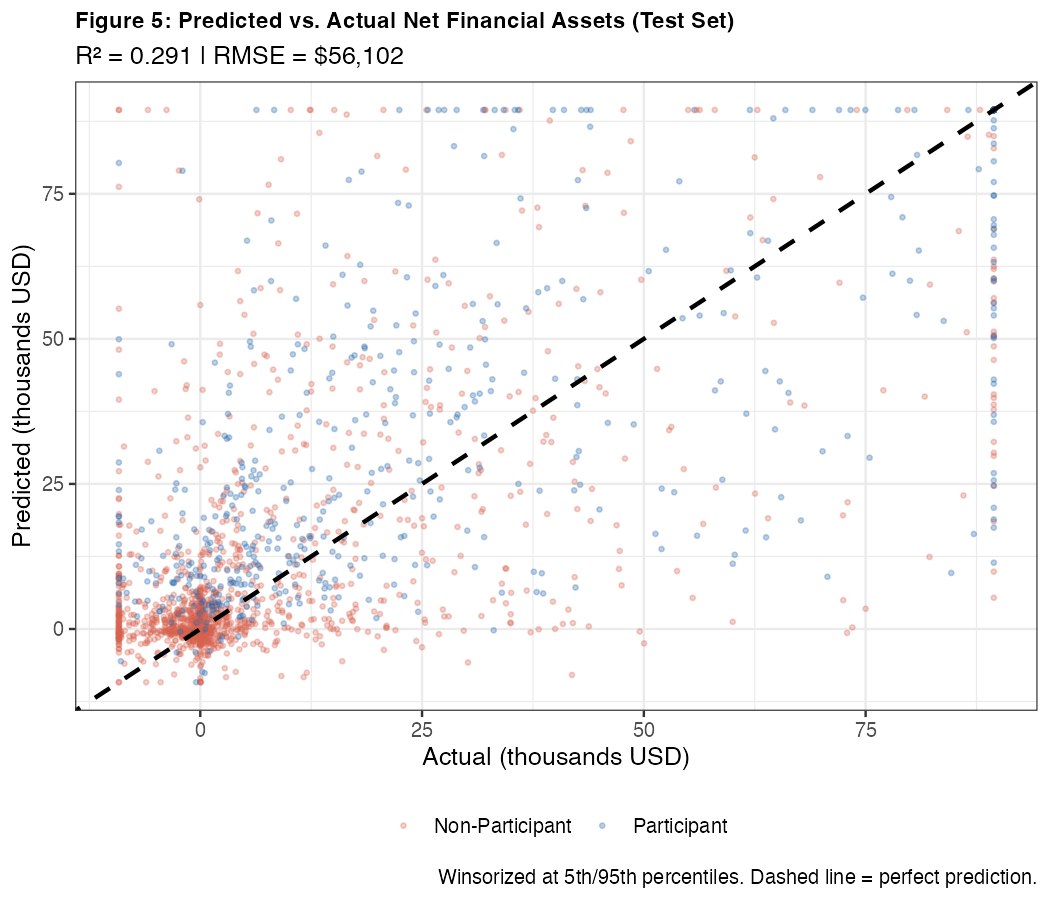
\includegraphics[width=0.7\linewidth]{figure5_predicted_vs_actual.png}
  \caption{Predicted versus actual net financial assets on the held-out test
  set.  Both axes winsorised at the 5th and 95th percentiles for legibility;
  dashed line is the 45-degree line.  Source: 1991 SIPP, $n=1{,}983$.}
  \label{fig:fit}
\end{figure}

\subsection{Instrumental-forest estimates of the treatment effect}

Table~\ref{tab:ate} reports the average treatment effects estimated by the
instrumental forest.  The estimated effect of 401(k) participation is about
\$11{,}400 on net financial assets (s.e.\ \$1{,}600) and about \$9{,}700 on
total wealth (s.e.\ \$2{,}600).  Both are statistically significant at
conventional levels.  In magnitude, these are economically meaningful:
\$11{,}400 corresponds to roughly two-thirds of the mean stock of net
financial assets in the full sample.

\begin{table}[H]
  \centering
  \caption{Average treatment effect of 401(k) participation, instrumental forest.}
  \label{tab:ate}
  \begin{tabular}{l S[table-format=6.0] S[table-format=4.0]}
    \toprule
    Outcome & {ATE (\$)} & {Std.\ Err.\ (\$)} \\
    \midrule
    Net financial assets & 11356 & 1621 \\
    Total wealth         &  9747 & 2636 \\
    \bottomrule
  \end{tabular}
  \par\smallskip
  \footnotesize
  \textit{Notes.}  Estimates from the instrumental forest of
  \cite{athey2019grf}, with \texttt{p401} as the treatment, \texttt{e401} as
  the instrument, and the covariates listed in Section~\ref{sec:data} as
  features.  Two thousand trees, automatically tuned splitting parameters.
  Test sample $n = 1{,}983$.
\end{table}

\subsection{Heterogeneity}

Figure~\ref{fig:hetinc} plots the mean of the individual treatment-effect
estimates by income bracket, with 95\% confidence intervals from the
within-group standard error.  The estimated effect on net financial assets
rises sharply with income, from about \$9{,}400 in the lowest bracket to
about \$21{,}100 in the highest.  Figure~\ref{fig:heteduc} shows a milder
gradient by education: mean treatment effects move from \$11{,}200 for
households with less than a high-school education to \$14{,}500 for those
with a college degree or more.  The age gradient (not shown as a separate
figure) is hump-shaped, peaking at \$15{,}600 for the 45--54 bracket.
Crucially, the effect is positive for every subgroup, and 100\% of test-set
$\hat\tau_i$ values are positive (see Figure~\ref{fig:tedist}).  This
suggests that, at least within the support of our covariates, 401(k)
participation never reduces net financial assets.

\begin{figure}[H]
  \centering
  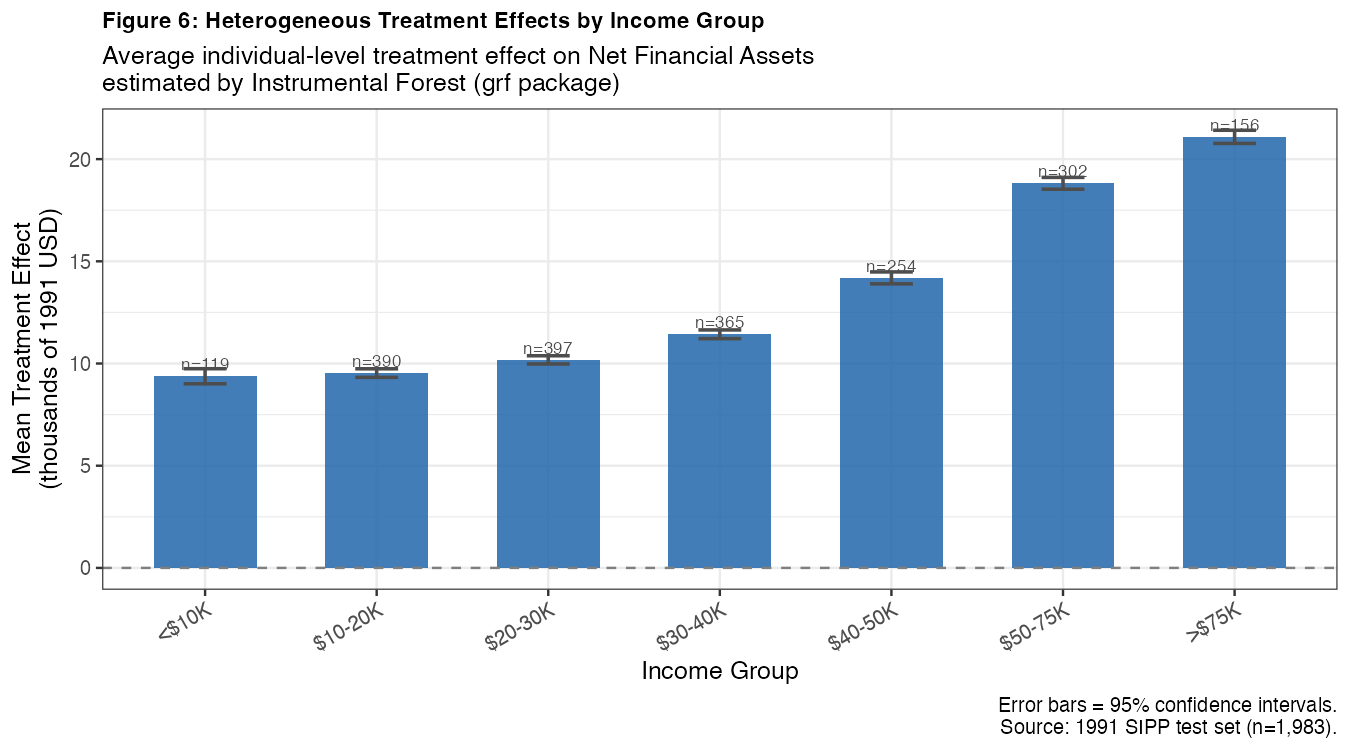
\includegraphics[width=0.85\linewidth]{figure6_heterogeneity_income.png}
  \caption{Heterogeneous treatment effects by income bracket.  Bars are
  group means of individual-level $\hat\tau_i$ from the instrumental
  forest; whiskers are 95\% CIs.}
  \label{fig:hetinc}
\end{figure}

\begin{figure}[H]
  \centering
  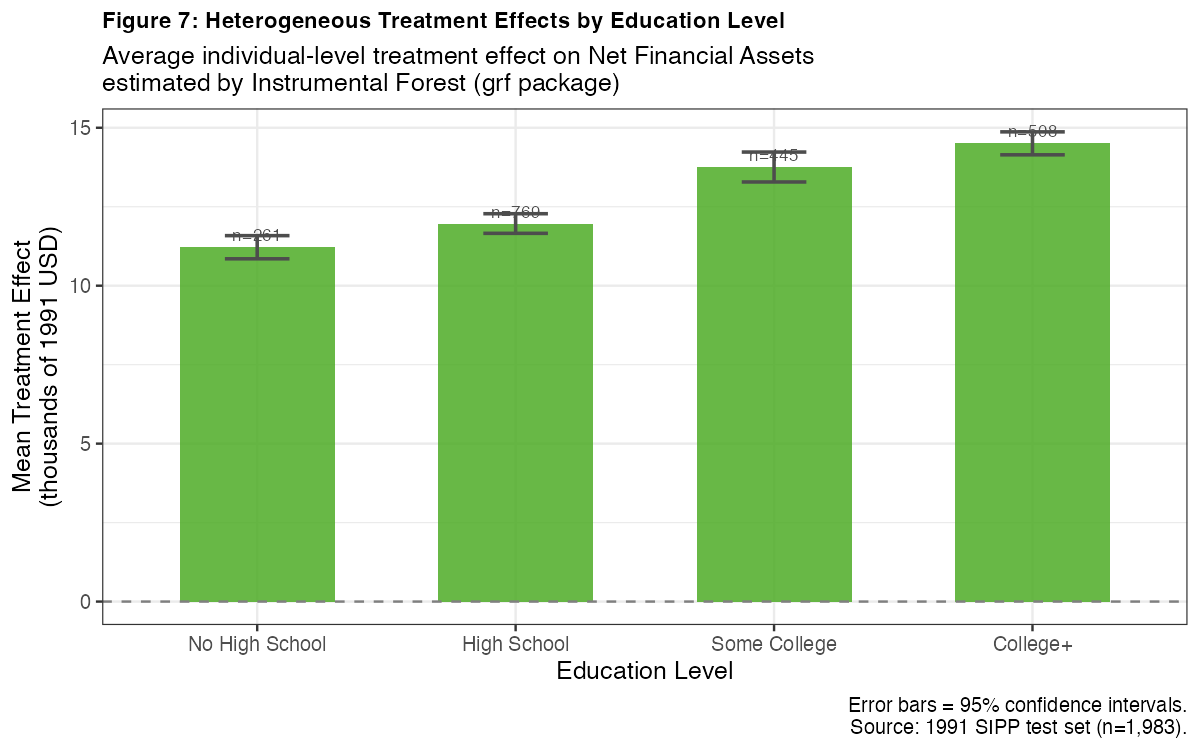
\includegraphics[width=0.78\linewidth]{figure7_heterogeneity_education.png}
  \caption{Heterogeneous treatment effects by education category.  Bars are
  group means of individual-level $\hat\tau_i$ from the instrumental
  forest; whiskers are 95\% CIs.}
  \label{fig:heteduc}
\end{figure}

\begin{figure}[H]
  \centering
  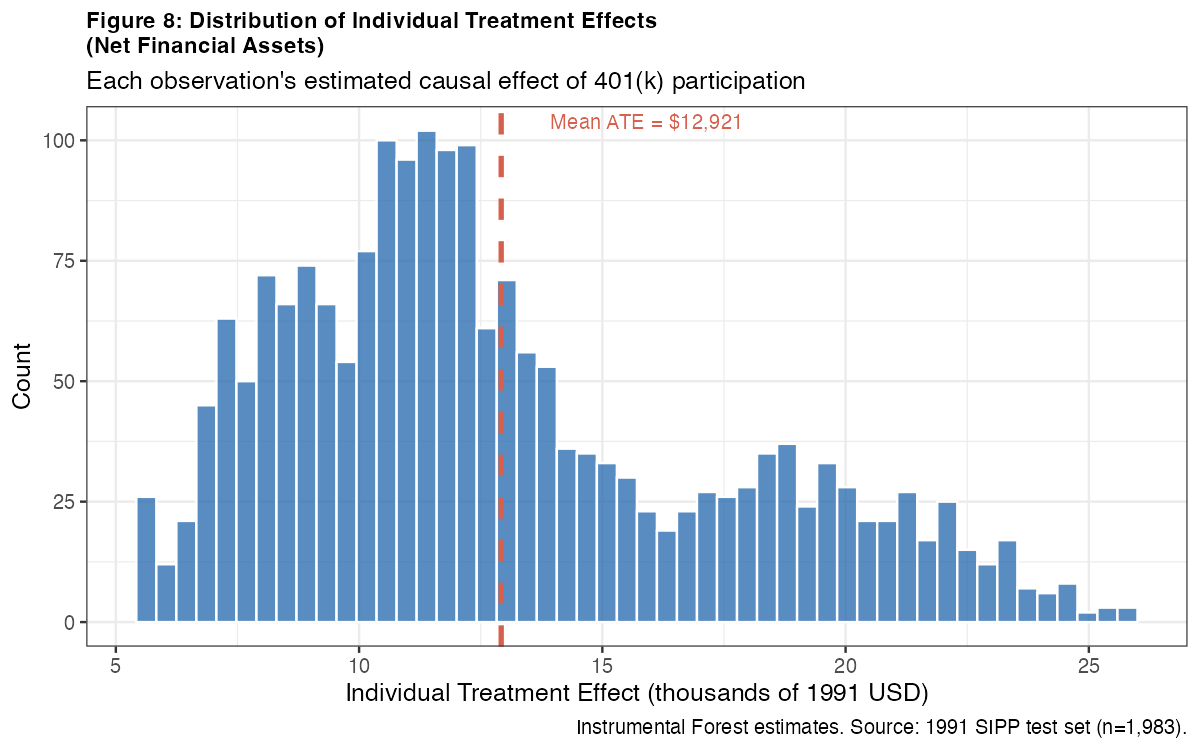
\includegraphics[width=0.78\linewidth]{figure8_te_distribution.png}
  \caption{Distribution of individual treatment-effect estimates
  $\hat\tau_i$ from the instrumental forest, net financial assets, test set.}
  \label{fig:tedist}
\end{figure}

A natural follow-up question is whether higher-income participants are
genuinely accumulating new wealth or shifting it from other accounts.
Figure~\ref{fig:nfavstw} compares treatment effects on net financial assets
and total wealth by income bracket.  Up to about the \$40{,}000 income
threshold, the two effects are similar in magnitude --- consistent with the
401(k) representing genuinely \emph{new} saving for these households.  In
the top two income brackets, the effect on net financial assets exceeds the
effect on total wealth, which is exactly the pattern one would expect if
high-income households partially substitute toward 401(k) wealth from other
forms of wealth (housing, taxable investments) rather than saving more
overall.  This echoes the asset-substitution finding that
\cite{ch2004} document at the upper quantiles of the wealth distribution.

\begin{figure}[H]
  \centering
  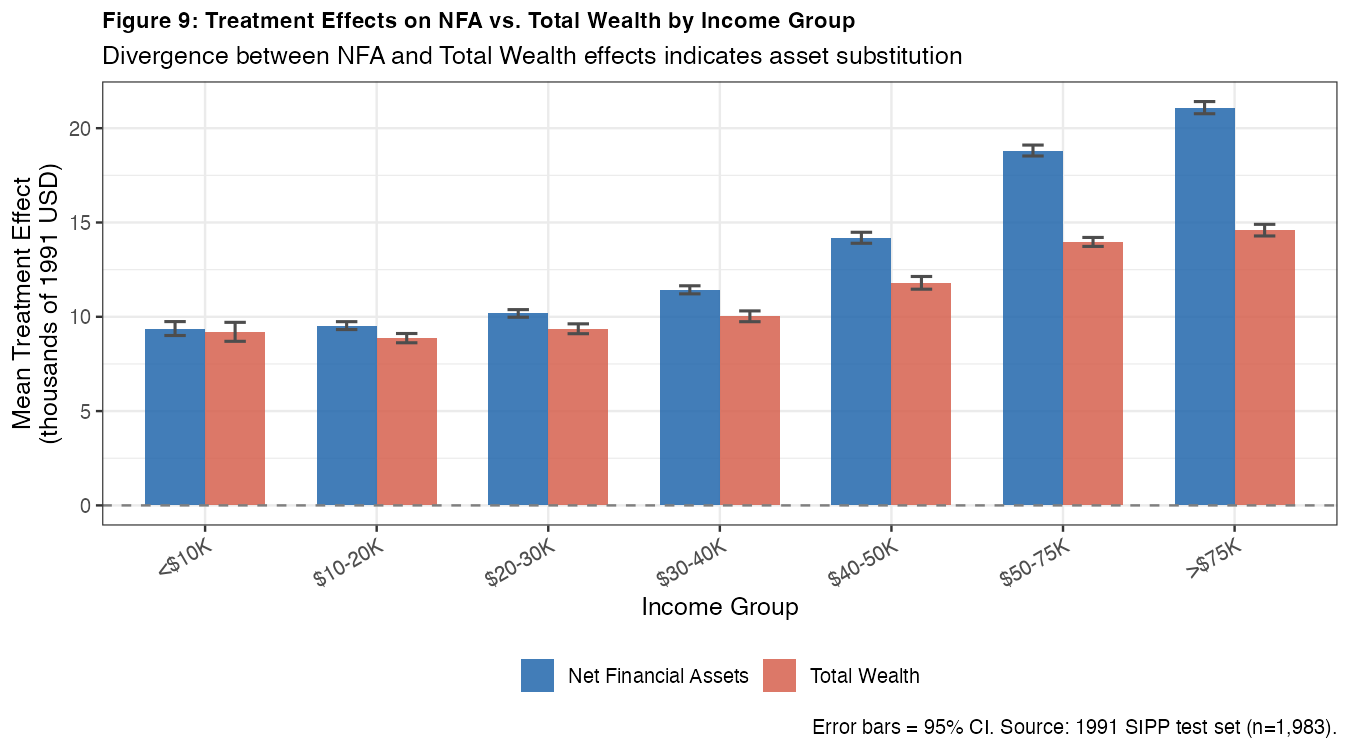
\includegraphics[width=0.85\linewidth]{figure9_nfa_vs_tw_by_income.png}
  \caption{Treatment effects on net financial assets versus total wealth by
  income bracket.  The widening gap at high incomes is consistent with
  asset substitution.}
  \label{fig:nfavstw}
\end{figure}

\subsection{Replication of \cite{ch2004} Table~3, Panel~A}

Table~\ref{tab:rep} reports the OLS and 2SLS estimates of the effect of
401(k) participation on each wealth measure, full sample and within each of
the seven income brackets.  As expected, the OLS estimates are uniformly
larger than the 2SLS estimates --- consistent with positive selection on
unobserved saving preference --- and the gap is largest where one would
expect the strongest selection (the upper income brackets).

The full-sample 2SLS estimate on net financial assets is \$13{,}087, with a
robust standard error of \$1{,}922 (compare to the OLS estimate of
\$14{,}520, s.e.\ \$1{,}551).  On net non-401(k) financial assets the 2SLS
point estimate is essentially zero (\$-220, s.e.\ \$1{,}803), implying that
the 401(k) gain shows up primarily as new financial wealth rather than as
substitution out of other financial accounts when averaged over the full
distribution.  On total wealth the 2SLS estimate is \$9{,}259 (s.e.\
\$3{,}035).

The lowest income bracket ($<\!\$10$K) is omitted because all
non-participants in that bracket are also ineligible, leaving the instrument
without variation; we report the bracket but the IV estimate is unreliable.

\begin{table}[H]
  \centering
  \caption{Replication of Table~3 Panel~A of \cite{ch2004}: OLS and 2SLS
  estimates of the effect of 401(k) participation, by income bracket.}
  \label{tab:rep}
  \footnotesize
  \begin{tabular}{l c r r r r r r}
    \toprule
    & & \multicolumn{2}{c}{Net financial assets} & \multicolumn{2}{c}{Net non-401(k) FA} & \multicolumn{2}{c}{Total wealth} \\
    \cmidrule(lr){3-4}\cmidrule(lr){5-6}\cmidrule(lr){7-8}
    Sample & $N$ & {OLS} & {2SLS} & {OLS} & {2SLS} & {OLS} & {2SLS} \\
    \midrule
    Full sample
      & 9{,}915 & 14{,}520 & 13{,}087 &      677 &     -220 & 10{,}694 &  9{,}259 \\
      &         & (1{,}551)& (1{,}922)& (1{,}434)& (1{,}803)& (2{,}388)& (3{,}035)\\[2pt]
    $<\!\$10$K\,$^\dagger$
      &    638 &  9{,}843 &  9{,}149 &  3{,}956 &  3{,}271 & 20{,}464 & 17{,}224 \\
      &        & (4{,}921)& (4{,}914)& (3{,}419)& (3{,}483)&(11{,}311)&(11{,}518)\\[2pt]
    \$10--20K
      & 1{,}948 &  5{,}591 &  5{,}352 &     -595 &     -918 &  4{,}729 &  6{,}138 \\
      &         & (1{,}463)& (1{,}629)& (1{,}216)& (1{,}397)& (2{,}265)& (3{,}218)\\[2pt]
    \$20--30K
      & 2{,}074 &  7{,}083 &  4{,}143 &      654 & -2{,}647 &  5{,}462 &        0 \\
      &         & (1{,}315)& (2{,}268)& (1{,}064)& (2{,}098)& (3{,}119)& (4{,}502)\\[2pt]
    \$30--40K
      & 1{,}712 & 12{,}136 & 10{,}273 &  1{,}424 &      -84 & 10{,}683 &  4{,}881 \\
      &         & (2{,}513)& (2{,}880)& (2{,}259)& (2{,}608)& (3{,}891)& (5{,}103)\\[2pt]
    \$40--50K
      & 1{,}204 & 12{,}858 &  9{,}980 &      466 & -2{,}174 & 13{,}470 & 13{,}205 \\
      &         & (2{,}470)& (3{,}741)& (2{,}232)& (3{,}528)& (4{,}905)& (6{,}675)\\[2pt]
    \$50--75K
      & 1{,}572 & 20{,}800 & 21{,}920 &  1{,}753 &  3{,}569 & 12{,}281 & 12{,}202 \\
      &         & (3{,}010)& (3{,}444)& (2{,}742)& (3{,}119)& (5{,}132)& (6{,}718)\\[2pt]
    $>\!\$75$K
      &    767 & 23{,}104 & 24{,}013 & -7{,}453 & -5{,}592 &  5{,}514 & 10{,}470 \\
      &        &(10{,}417)&(12{,}895)&(10{,}047)&(12{,}518)&(13{,}645)&(17{,}174)\\
    \bottomrule
  \end{tabular}
  \par\smallskip
  \footnotesize
  \textit{Notes.}  Robust (HC1) standard errors in parentheses.  Outcomes
  are net financial assets (\texttt{net\_tfa}), net non-401(k) financial
  assets (\texttt{net\_nifa}) and total wealth (\texttt{tw}), all in 1991
  dollars.  OLS specification: equation (\ref{eq:ols}).  2SLS specification:
  equation (\ref{eq:2sls}), using \texttt{e401} as an instrument for
  \texttt{p401}.  Within-bracket regressions include income linearly and
  drop the income-bracket dummies; full-sample regressions include both.
  $^\dagger$ In the lowest income bracket, all non-participants are
  ineligible for a 401(k), so the instrument has limited variation; the IV
  estimate in that row should be interpreted with caution.
\end{table}

\paragraph{Pattern across income brackets.}
Both OLS and 2SLS estimates rise with income, mirroring the pattern in
Figure~\ref{fig:hetinc}.  The 2SLS estimates on net non-401(k) financial
assets are negative in several brackets and increasingly so toward the top,
again consistent with substitution.  Figure~\ref{fig:olsiv} plots the
within-bracket OLS and 2SLS coefficients side by side.

\begin{figure}[H]
  \centering
  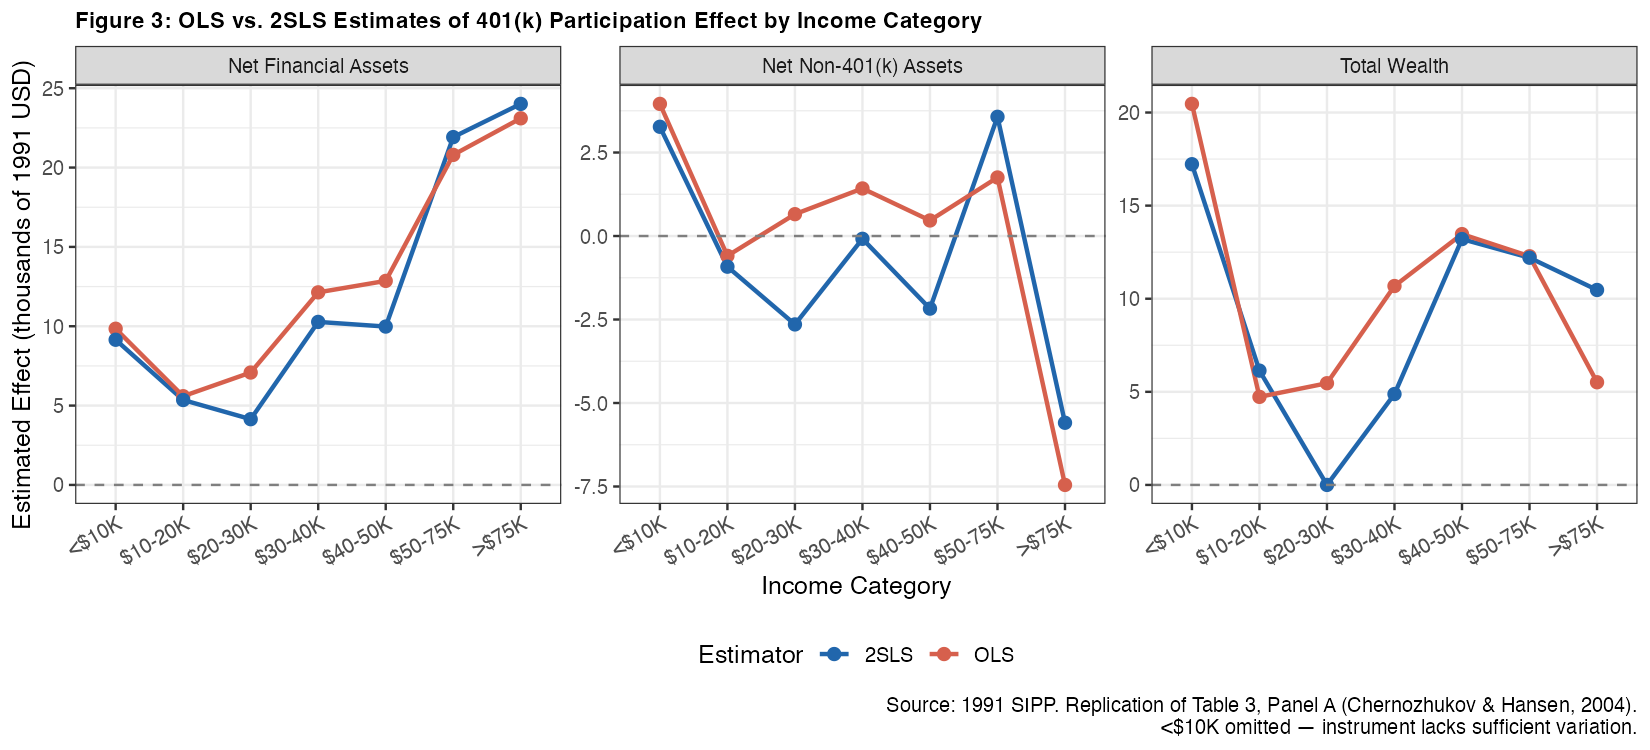
\includegraphics[width=0.95\linewidth]{figure3_ols_vs_2sls.png}
  \caption{OLS and 2SLS estimates of the effect of 401(k) participation by
  income bracket (replication of Table~3 Panel~A of \citealp{ch2004}, full
  sample omitted).  The lowest income bracket is dropped because of
  insufficient instrument variation.}
  \label{fig:olsiv}
\end{figure}

\subsection{Comparing the ML estimates to OLS and 2SLS}

The ML and 2SLS estimates tell a consistent story.  The instrumental
forest's full-sample ATE on net financial assets (\$11{,}356) sits between
the OLS estimate (\$14{,}520) and the 2SLS estimate (\$13{,}087), but is
much closer to 2SLS than to OLS.  On total wealth the ML estimate of
\$9{,}747 is essentially indistinguishable from the 2SLS estimate of
\$9{,}259.  Two observations follow.

First, the qualitative interpretation of the data does not depend on which
of these estimators one uses: 401(k) participation has a statistically and
economically significant positive effect on net financial assets, a smaller
positive effect on total wealth, and the difference between the two grows
at high incomes in a way that suggests asset substitution at the top.  This
is encouraging, because it means the headline conclusion is not an artefact
of any one method.

Second, both IV-based estimators land below the OLS estimates, in line with
the standard prior that workers with higher unobserved saving propensity
are more likely to participate.  The instrumental forest's advantage is not
that it produces a different ATE --- it does not --- but that it produces
\emph{individual-level} treatment-effect estimates and a covariate-adaptive
specification, which is what makes the heterogeneity analysis in
Section~4.3 possible without committing in advance to a particular set of
interaction terms.

\subsection{Strengths, weaknesses, and what would improve the model}

The main strengths of the approach are: (i) the use of an external
instrument addresses the central confounder in this literature
(unobserved preference for saving); (ii) the random forest captures
nonlinearities in the relationship between covariates and wealth that a
linear model cannot; and (iii) the instrumental forest delivers a flexible
ATE and individual-level $\hat\tau_i$ at the same time.

The main weaknesses are also worth being explicit about.  The $R^2$ of the
prediction model is modest, especially for net financial assets.  Wealth is
heavy-tailed and the SIPP records few of the variables that would best
explain the right tail (gifts, inheritances, business ownership history,
behavioural traits like patience or financial literacy).  More data --- in
particular a panel that lets us partial out fixed unobserved saving
preferences --- and richer covariates would help more than a more
sophisticated estimator on this same cross section.  Better compute would
mainly let us tune more aggressively and bootstrap the heterogeneity
results, but is unlikely to move the headline numbers.

The exclusion restriction for \texttt{e401} as an instrument is the
identifying assumption.  It can fail if employers who offer 401(k) plans
are systematically different from those who do not in ways that affect
worker wealth through channels other than 401(k) participation (e.g.\
better pension matches, higher wages conditional on observed
characteristics, or worker self-sorting across firms).  Conditional on the
income, education, and demographic covariates we control for, this is the
same assumption that \cite{ch2004}, \citet{poterba1995etal} and
\cite{abadie2003} all rely on; it is plausible but not testable directly.
Our estimates should therefore be interpreted as the local average effect
on \emph{compliers} --- workers whose participation status responds to
employer eligibility --- rather than a population-wide structural
parameter.

\section{Conclusion}\label{sec:conclusion}

We use the 1991 SIPP to estimate the causal effect of 401(k) participation
on three measures of household wealth, using 401(k) eligibility as an
instrument and an instrumental-forest estimator from \cite{athey2019grf}.
The estimated average treatment effect is around \$11{,}400 on net
financial assets and \$9{,}700 on total wealth, in close agreement with the
2SLS estimates from a replication of Panel~A of Table~3 of \cite{ch2004}.
Effects are positive for every income, education and age subgroup we
examine, but they rise sharply with income, and the divergence between net
financial assets and total wealth at high incomes is consistent with
asset substitution.

The agreement between the parametric IV estimates and the ML-based
estimates is itself informative.  When the underlying causal model is
relatively simple --- one binary treatment, one binary instrument, a modest
number of covariates --- a flexible non-parametric estimator does not
overturn the linear IV result; rather it lets us interrogate the
heterogeneity that the linear specification has to assume away.  We see
this as a useful template more broadly: ML methods are most valuable here
not for changing the headline estimate but for documenting where it varies.

Several caveats apply.  Because we use a single cross-section, we cannot
control for time-invariant unobserved heterogeneity in saving preference
beyond what the instrument removes.  The exclusion restriction is
defensible but not testable.  The estimates apply to compliers, and the
top income brackets in particular contain few non-eligibles, making
inference there imprecise.  Future work could exploit the panel structure
of the SIPP, control directly for measures of financial literacy or
intertemporal preference where available, and extend the analysis to
quantile treatment effects in the spirit of the original
\cite{ch2004} paper.

\renewcommand{\refname}{References}
\begin{thebibliography}{99}

\bibitem[Abadie(2003)]{abadie2003}
Abadie, Alberto.
``Semiparametric Instrumental Variable Estimation of Treatment Response
Models.''
\emph{Journal of Econometrics} 113, no.~2 (2003): 231--263.

\bibitem[Athey, Tibshirani, and Wager(2019)]{athey2019grf}
Athey, Susan, Julie Tibshirani, and Stefan Wager.
``Generalized Random Forests.''
\emph{Annals of Statistics} 47, no.~2 (2019): 1148--1178.

\bibitem[Chernozhukov and Hansen(2004)]{ch2004}
Chernozhukov, Victor, and Christian Hansen.
``The Effects of 401(k) Participation on the Wealth Distribution: An
Instrumental Quantile Regression Analysis.''
\emph{Review of Economics and Statistics} 86, no.~3 (2004): 735--751.

\bibitem[Poterba, Venti, and Wise(1995)]{poterba1995etal}
Poterba, James M., Steven F. Venti, and David A. Wise.
``Do 401(k) Contributions Crowd Out Other Personal Saving?''
\emph{Journal of Public Economics} 58, no.~1 (1995): 1--32.

\end{thebibliography}

\end{document}
